
\chapter{Besoins et objectifs}

\section{Origine du besoin}

L'objectif de ce projet est de développer un programme d’apprentissage par renforcement capable de jouer à un jeu, dans le cadre de l’UE Projet de L3 informatique. 
\par
Le choix du jeu en question ainsi que des algorithmes utilisés reste libre, cependant l'énoncé original du sujet mentionnait Pac-Man ainsi que Space Invaders comme jeux possibles (modifié depuis pour n'inclure que la recherche de trésor et le Tic-tac-toe). Ces exemples de jeux ont éveillé notre curiosité sur le sujet, et nous avons donc décidé de tenter d'appliquer l'apprentissage par renforcement sur Pac-Man, qui est un jeu relativement complexe.
\par
Toutefois suite aux conseils du professeur référent et aux recherches de solutions à ce problème, nous avons pris conscience de la difficulté du projet. Nous avons en conséquence décidé d'appliquer dans un premier temps l'apprentissage par renforcement sur la recherche de trésor, un jeu extrêmement basique, afin d'en acquérir les bases et les concepts. Une fois cette étape franchie, nous pourrions nous attarder sur le plus complexe : Pac-Man.

\section{Principe du jeu ``Recherche de trésor''}

Le jeu “Recherche de trésor” est un jeu simple où il est possible de déplacer case par case un personnage dans un espace en une ou deux dimensions, et dont le but est d’arriver jusqu’à un trésor. En deux dimensions, il est aussi possible d’ajouter des murs et des obstacles afin de complexifier la tâche. 
\par
Ce jeu ne possède aucune difficulté particulière, spécialement en une dimension où le personnage n'a qu'à avancer à répétition dans la bonne direction jusqu'au trésor.
\par
En deux dimensions, l'agent devra mémoriser le chemin à emprunter pour arriver jusqu'au trésor.

\section{Principe de Pac-Man}
Pac-Man est un jeu d’arcade sorti en 1980 où l’on dirige le personnage éponyme dans un labyrinthe rempli d’objets à ramasser, l’objectif étant de ramasser toutes les “pac-gommes” pour passer au niveau suivant.
Pour complexifier la tâche, 4 fantômes rôdent dans le labyrinthe, et font perdre une vie à Pac-Man (qui en possède 3) au moindre contact . Il est temporairement possible de pouvoir les éliminer en ramassant certains objets, mais les fantômes finiront par réapparaître.
\par
Chacun des 4 fantômes a un comportement différent :

\begin{itemize}
	\item Le rouge suit Pac-Man à la trace
	\item Le rose et le bleu essayent de couper la route à Pac-Man en se plaçant devant lui
	\item Le orange se déplace aléatoirement
\end{itemize}


\section{Principe de l’apprentissage par renforcement}

L’apprentissage par renforcement est une méthode d’apprentissage où un \textbf{agent} logiciel autonome doit apprendre quelles actions effectuer dans un \textbf{environnement} donné, de façon à obtenir la plus grande récompense possible.\par

Ce genre d’algorithme fonctionne généralement à l’aide de 3 entités : 
\begin{itemize}
	\item Un agent, qui va prendre les décisions et effectuer des actions
	\item Un environnement, sur lequel l’agent agira
	\item Une interface, qui se chargera de fournir les informations actuelles sur l’environnement à l’agent (image, son, données numériques, etc) ainsi que la ``récompense'' associée à chaque action effectuée.
\end{itemize}

On désigne par récompense une valeur numérique arbitraire indiquant la qualité de l'action effectuée. Une récompense positive est associée à un comportement désiré menant à la victoire (augmenter le score, avancer dans le niveau, se rapprocher d'un objet, etc), tandis qu'une récompense négative est associée à un comportement néfaste à l'objectif visé (perdre une vie, prendre des dégats, etc).
Ici, l’environnement sera un jeu Pac-Man standard, et l’agent se substituera au joueur pour y jouer.


\section{Moyens et contraintes}
\subsection{Moyens financiers}
Le cadre dans lequel nous réalisons ce projet ne permet pas d’obtenir un budget pour son développement. Toutefois, ce dernier ne devrait pas nécessiter de dépense, et s’appuiera sur des technologies et ressources libres de droit.

\subsection{Moyens humains}
L’unique équipe derrière ce produit est constitué du binôme d’étudiants en charge du projet (Alexis PLAQUET et Tom RIVERO). Il est cependant possible d’obtenir de l’aide et des renseignements auprès des professeurs chargés d’assurer l’UE Projet.

\section{Modalités de mise en oeuvre}
Le client requiert seulement que le programme soit utilisable sous Linux.



\chapter{Analyse de l’existant, concurrence et positionnement}

\section{Description de l’existant}
Ce projet n’a pas pour objectif d’être novateur, il est en effet courant de tester des algorithmes d’apprentissage par renforcement sur des jeux vidéos, notamment parce que ces derniers sont facilement compréhensible pour les humains, que la lecture de l’écran de jeu est plus simple et intéressante qu’avec des jeux plus théoriques, et qu’il est aisé de comparer les performances d’une intelligence artificielle à celles d’un humain.

\section{Analyse de l’existant}
\subsection{Maluuba}
Le projet de faire jouer une intelligence artificielle à Pac-Man a été complètement accompli en 2017 par Maluuba \cite{maluuba}.
Maluuba a développé un agent utilisant utilise des techniques bien au delà des moyens de ce projet, comme la Hybrid Reward Architecture, afin d'atteindre le score maximal possible sur Pac-Man \cite{hra}.

\subsection{Projets amateurs}
De par la popularité d'OpenAI Gym, une librairie offrant de nombreux environnements (dont des jeux), on retrouve évidemment des projets identiques au nôtre. Ces derniers sont souvent des projets amateurs, des projets universitaires, et des projets effectués dans le cadre de recherches. La grande majorité est d’excellente qualité et la plupart bien documentée \cite{pacmanai1,pacmanai2,pacmanai3}.


\section{Positionnement par rapport à l'existant}
Comme évoqué précédemment, les objectifs que nous nous sommes fixés ont déjà été accomplis par d’autres personnes, et il paraît peu réaliste d’imaginer un projet dans ce domaine et avec nos compétences actuelles qui serait novateur.
\par
Le but principal de ce projet est avant tout de nous permettre de comprendre et d’appliquer la théorie et les algorithmes derrière l’apprentissage par renforcement.

\section{Cible du produit}
Sont ciblées principalement les personnes intéressées par l’apprentissage par renforcement. Celles-ci devront être capable d’installer d’elles même les librairies ou logiciels nécessaire à l'exécution de l’algorithme. Bien que ce rapport soit en français, l'entièreté du code ainsi que ses commentaires seront en anglais afin de permettre sa compréhension au plus grand nombre.
\par
Enfin, il est à noter que ce projet ne fera pas l’objet d’efforts d’accessibilité, il sera donc probablement inutilisable pour un usager malvoyant par exemple.


\chapter{Offre fonctionnelle}
\section{Fonctions principales}
Le logiciel disposera de trois modes principaux : entraînement, visualisation et tests. \par

On pourra ainsi entraîner un agent choisi, c’est à dire le laisser en phase d’apprentissage afin qu’il améliore la prédiction des actions à effectuer et apprenne à jouer
\par
La visualisation permet de voir de façon graphique comment l’IA joue, on pourra contrôler la vitesse d’affichage du jeu (afficher le jeu en ralenti ou en accéléré).
\par
Enfin, le mode test permettra de lancer une série de simulations pour voir quel score l’IA obtient en moyenne, le pourcentage d'échec, ainsi que toute autre statistique utile permettant d’évaluer la qualité de l’IA actuelle.

\section{Fonctions optionnelles}
Bien que intéressantes et utiles dans le cadre du projet, ces fonctionnalités pourraient être coûteuses en temps d’implémentation. \par

Au démarrage du logiciel, l’utilisateur pourra sélectionner sur quel jeu ou simulation il souhaite faire travailler l’apprentissage par renforcement, il pourra alors choisir parmi une liste prédéterminée. \par
Une fois ceci fait, l’utilisateur pourra choisir avec quel type d’algorithme d’apprentissage par renforcement il souhaite travailler, puis si cela a un sens dans le contexte de l’algorithme, choisir les paramètres de ce dernier. A ce moment il sera aussi possible à l’utilisateur de choisir de charger une sauvegarde existante de l’IA entraînée s’il en existe. L’utilisateur pouvant sauvegarder son IA après chaque entraînement. \par
Il serait aussi possible à l’utilisateur de jouer lui-même au jeu qu’il a sélectionné, si cela est humainement possible (cela pourrait ne pas l’être dans le cadre de certaines simulations).
\par
Il est aussi envisageable d'ajouter une interface graphique permettant de contrôler le tout de façon plus intuitive et rapide.


\section{Description fonctionnelle}

%---Entrainer---
\begin{center}
\begin{tabularx}{\linewidth}{|p{2.8cm}|X|}
    \hline
	\multicolumn{2}{|c|}{\textbf{Entrainer l'agent}}\\
	\hline
	\hline
	Description &
	Lance l'apprentissage de l'agent selon des paramètres donnés. \\
	\hline
	Paramètres d'entrée &
	\begin{minipage}[t]{\linewidth}
    \begin{itemize}[nosep,after=\strut,leftmargin=*]
        \item Nombre d'épisodes
        \item Affichage ou non des informations au fil de l'entraînement
        \item Paramètres spécifiques à chaque type d’algorithme d’apprentissage par renforcement
    \end{itemize}
    \end{minipage}
    \\ 
	\hline
	Paramètres de sortie &
	La structure de donnée de l'agent une fois entraîné\\
	\hline
	Contraintes à vérifier avant l'exécution &
	Le nombre d'épisode doit être un entier strictement positif \\
	\hline
	En cas d'erreur &
	Arrêter l'entraînement et en informer l’utilisateur \\
	\hline
	Priorité &
	Must \\
	\hline
\end{tabularx}
\end{center}

\vspace*{1 cm}

%---Tester---
\begin{center}
\begin{tabulary}{1.0\textwidth}{|L | L |}
	\hline
	\multicolumn{2}{|c|}{\textbf{Tester l'agent}}\\
	\hline
	\hline
	Description &
	Laisse l'agent compléter un nombre d’épisodes donné et calcule les statistiques de victoire, la moyenne d’actions nécessaires pour gagner une partie, etc\\
	\hline
	Paramètres d'entrée &
	\begin{minipage}[t]{\linewidth}
    \begin{itemize}[nosep,after=\strut,leftmargin=*]
        \item Nombre d'épisodes
    \end{itemize}
    \end{minipage}
    \\
	\hline
	Paramètres de sortie &
	Les données et statistiques résultant des tests\\
	\hline
	Contraintes à vérifier avant l'exécution &
	Le nombre d’épisodes doit être un entier strictement positif \\
	\hline
	En cas d'erreur &
	Arrêter le test, en informer l’utilisateur \\
	\hline
	Priorité &
	Must \\
	\hline
\end{tabulary}
\end{center}

\vspace*{1 cm}

%---Regarder jouer---

\begin{center}
  \begin{tabularx}{\linewidth}{|p{2.8cm}|X|}
    \hline
	\multicolumn{2}{|c|}{\textbf{Regarder l’agent jouer}}\\
	\hline
	\hline
	Description &
	Lance la visualisation graphique de l’agent jouant en temps réel\\
	\hline
	Paramètres d'entrée &
	\begin{minipage}[t]{\linewidth}
    \begin{itemize}[nosep,after=\strut,leftmargin=*]
        \item Vitesse de lecture
        \item Nombre de parties
    \end{itemize}
    \end{minipage}
    \\ 
	\hline
	Paramètres de sortie &
	Affichage graphique du jeu\\
	\hline
	Contraintes à vérifier avant l'exécution &
	La vitesse de lecture doit être un réel strictement positif et le nombre d’épisodes doit être un entier strictement positif \\
	\hline
	En cas d'erreur &
	Arrêter la lecture, en informer l’utilisateur \\
	\hline
	Priorité &
	Should \\
	\hline
  \end{tabularx}
\end{center}

\vspace*{1 cm}

%---Sauvegarder---

\begin{center}
  \begin{tabularx}{\linewidth}{|p{2.8cm}|X|}
    \hline
	\multicolumn{2}{|c|}{\textbf{Sauvegarder l'agent}}\\
	\hline
	\hline
	Description &
	Permet de sauvegarder l’état actuel de l’IA utilisée\\
	\hline
	Paramètres d'entrée &
	\begin{minipage}[t]{\linewidth}
    \begin{itemize}[nosep,after=\strut,leftmargin=*]
        \item Nom du fichier
    \end{itemize}
    \end{minipage}
    \\ 
	\hline
	Paramètres de sortie &
	Le fichier sauvegardé\\
	\hline
	Contraintes à vérifier avant l'exécution &
	Avoir les droits d’écriture sur le nom du fichier donné \\
	\hline
	En cas d'erreur &
	Informer l’utilisateur que le fichier n’a pas pu être sauvegardé \\
	\hline
	Priorité &
	Should \\
	\hline
  \end{tabularx}
\end{center}

\vspace*{1 cm}

%---Charger---

\begin{center}
  \begin{tabularx}{\linewidth}{|p{2.8cm}|X|}
    \hline
	\multicolumn{2}{|c|}{\textbf{Charger l'agent}}\\
	\hline
	\hline
	Description &
	Permet de charger depuis le disque dur une IA précédemment sauvegardée\\
	\hline
	Paramètres d'entrée &
	\begin{minipage}[t]{\linewidth}
    \begin{itemize}[nosep,after=\strut,leftmargin=*]
        \item Nom du fichier
    \end{itemize}
    \end{minipage}
    \\ 
	\hline
	Paramètres de sortie &
	L’IA chargée\\
	\hline
	Contraintes à vérifier avant l'exécution &
	Avoir les droits de lecture sur le nom du fichier donné \\
	\hline
	En cas d'erreur &
	Informer l’utilisateur que le fichier n’a pas pu être chargé \\
	\hline
	Priorité &
	Should \\
	\hline
  \end{tabularx}
\end{center}

\vspace*{1 cm}


%---Selectionner jeu---

\begin{center}
  \begin{tabularx}{\linewidth}{|p{2.8cm}|X|}
    \hline
	\multicolumn{2}{|c|}{\textbf{Sélectionner l'environnement}}\\
	\hline
	\hline
	Description &
	Permet de sélectionner le jeu ou la simulation sur laquelle on souhaite faire travailler l’IA\\
	\hline
	Paramètres d'entrée &
	\begin{minipage}[t]{\linewidth}
    \begin{itemize}[nosep,after=\strut,leftmargin=*]
        \item Nom du jeu
    \end{itemize}
    \end{minipage}
    \\ 
	\hline
	Paramètres de sortie &
	\\
	\hline
	Contraintes à vérifier avant l'exécution &
	Le jeu doit exister dans la base de données \\
	\hline
	En cas d'erreur &
    Informer l’utilisateur que le jeu n’est pas valide ou qu’une erreur s’est produite lors de son chargement \\
	\hline
	Priorité &
	Could \\
	\hline
  \end{tabularx}
\end{center}

\vspace*{1 cm}

%---Selectionner jeu---

\begin{center}
  \begin{tabularx}{\linewidth}{|p{2.8cm}|X|}
    \hline
	\multicolumn{2}{|c|}{\textbf{Sélectionner un type d’algorithme d’apprentissage par renforcement
}}\\
	\hline
	\hline
	Description &
	Permet de sélectionner un type d’algorithme avec lequel travailler\\
	\hline
	Paramètres d'entrée &
	\begin{minipage}[t]{\linewidth}
    \begin{itemize}[nosep,after=\strut,leftmargin=*]
        \item Le type d’algorithme
        \item Les paramètres requis par l’algorithme
    \end{itemize}
    \end{minipage}
    \\ 
	\hline
	Paramètres de sortie &
	Un agent de l’algorithme demandé
	\\
	\hline
	Contraintes à vérifier avant l'exécution &
	Le type d’algorithme doit exister et les paramètres doivent être valides \\
	\hline
	En cas d'erreur &
    Informer l’utilisateur que sa sélection est incorrecte
    \\
	\hline
	Priorité &
	Would \\
	\hline
  \end{tabularx}
\end{center}

%---Jouer au jeu---

\begin{center}
  \begin{tabularx}{\linewidth}{|p{2.8cm}|X|}
    \hline
	\multicolumn{2}{|c|}{\textbf{Laisser l'utilisateur jouer à l'environnement
}}\\
	\hline
	\hline
	Description &
	Permet de jouer manuellement au jeu ou à la simulation actuelle\\
	\hline
	Paramètres d'entrée & Jeu désiré
    \\ 
	\hline
	Paramètres de sortie &
	\\
	\hline
	Contraintes à vérifier avant l'exécution &
	Le jeu doit exister et pouvoir être jouable par un humain \\
	\hline
	En cas d'erreur &
    Informer l’utilisateur que sa sélection est incorrecte
    \\
	\hline
	Priorité &
	Would \\
	\hline
  \end{tabularx}
\end{center}

\chapter{Maquette et charte graphique}

L’IA sera exécutée depuis l’invite de commande, la seule interface graphique sera l’affichage du jeu.
Une charte graphique n'a donc pas lieu d'être.
L’utilisateur se verra présenter des menus à choix multiples ainsi que des entrées de textes afin de naviguer parmi les menus et définir les paramètres.
En voici des exemples permettant d’accéder aux différentes fonctionnalités précédemment introduites.

Au lancement du logiciel, l’utilisateur pourra choisir le type de jeu sur lequel travailler, puis une fois ce dernier choisi l’utilisateur devra choisir quel type d’apprentissage par renforcement il souhaite utiliser (il pourra aussi à ce moment choisir de jouer lui même au jeu)

\begin{center}
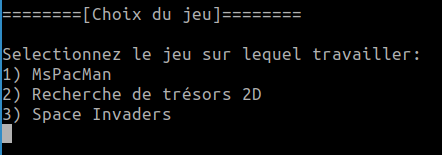
\includegraphics[width=0.5\textwidth]{maquette_choixjeu.png}
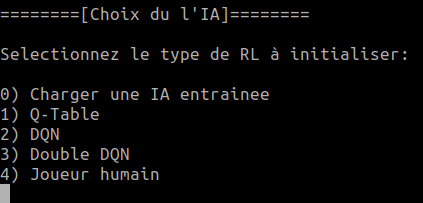
\includegraphics[width=0.5\textwidth]{maquette_choixia.png}
\end{center}

Dans le cas où le joueur choisit de charger une IA, la liste des IA précédemment sauvegardées sera affichée.

\begin{center}
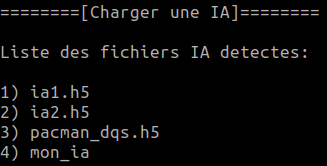
\includegraphics[width=0.5\textwidth]{maquette_chargeria.png}
\end{center}

Une fois l’IA choisie ou chargée, l’utilisateur arrive sur le menu principal où il peut sélectionner une action à effectuer sur l’IA.

\begin{center}
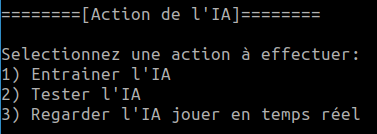
\includegraphics[width=0.5\textwidth]{maquette_actionia.png}
\end{center}

Dans le cas où l’utilisateur souhaite entraîner l’IA, il devra entrer plusieurs paramètres permettant de configurer cet entraînement.

\begin{center}
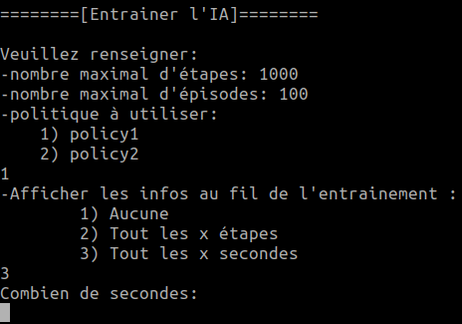
\includegraphics[width=0.5\textwidth]{maquette_entraineria.png}
\end{center}

Une fois l'entraînement de l’IA terminé, l'utilisateur a la possibilité de sauvegarder l’IA entraînée pour la réutiliser ultérieurement.

\begin{center}
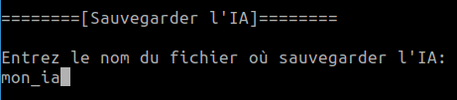
\includegraphics[width=0.5\textwidth]{maquette_sauvegarderia.png}
\end{center}

Enfin, si l’utilisateur désire voir l’IA jouer, il doit entrer quelques paramètres, et le jeu (joué par l’IA) sera affiché.

\begin{center}
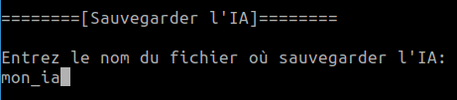
\includegraphics[width=0.5\textwidth]{maquette_sauvegarderia.png}
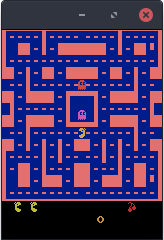
\includegraphics[width=0.5\textwidth]{maquette_mspacman.png}
\end{center}
